\section{Materials \& Methods}

\subsection{Macroevolutionary patterns of dietary evolution in marine fishes}

We used the {\tt R} package {\tt rfishbase} \cite{boettiger2012rfishbase} to obtain a list of all described species of marine spiny-finned (acanthopterygian) fish. We then used the package to obtain a depth range for marine pharyngognathous spiny-finned fishes. Numerous species occur in extremely shallow habitats, while the deepest recorded marine pharyngognath was {\em Bodianus cylindriatus}, listed as occurring down to 510m.

We then compiled volumetric gut contents for all fishes in {\tt Fishbase}. \cite{froese2013fishbase} Fishbase lists four potential ontogenetic stages for marine fish in diet studies, larvae, newly settled larvae (recruits), juveniles, and adults. We only used dietary studies involving juveniles and adult fish, never larvae or the newly settled recruits. Dietary data was compiled into three categories: piscivory (non-larval fish), processing-intensive prey (hard-shelled prey, detritus, algae, plants). We also defined an `other' category made of all prey items not listed in the previous two categories (eg. zooplankton, soft-bodied invertebrates, mammals, etc). 

The degree of piscivory was defined as the volumetric percentage of non-larval fish in the diet, and the degree of processing-intensive prey was defined as the volumetric percentage of plants, algae, and detritus combined with the percentage of hard-shelled prey like bivalves, shelled gastropods, and hard-bodied echinoderms (ie. no holothurian ``sea cucumbers''). We analyzed herbivorous and hard-shelled prey as separate variables, but found no difference in overall results for any analysis, so they were left together. If multiple diet studies for a species were available, the mean values for each category were weighted by the number of fish in each study. Studies with no sample size listed were downweighted compared to studies with known sample sizes by treating a lack of listed sample size as equivalent to $N=1$.

We then reduced our diet dataset (n=1937) down to marine spiny-finned fishes (n=1288) found at the appropriate depth (n=1285) for which phylogenetic information \cite{rabosky2013rates} was available (n=853). Two species, the grouper Cephalopholis argus and the rabbitfish Siganus rivulatus were incorrectly placed within Labridae in the original Rabosky tree, \cite{rabosky2013rates} so we removed them prior to additional analysis. In total, this gave us a dataset of 851 species, including representatives from all four major marine pharyngognath lineages. We mapped pharyngognathy at the base of Labridae/Scaridae/Odacidae, Pomacentridae, Exocetidae/Hemirhampidae, and Embiotocidae, as mapped in a previous study. \cite{wainwright_evolution_2012} We used the {\tt brownie.lite} function in the {\tt phytools} \cite{revell2012phytools} {\tt R} package to test whether each diet category was best modeled as a one-rate model across the tree, or a model where rates differed between pharyngognathous and non-pharyngognathous marine fishes. There was a strong preference for a two-rate model for both fish prey($\Delta$AICc = -293, Table \ref{FJ_table1}) and processing-intensive prey($\Delta$AICc = -59, Table \ref{FJ_table1}). For both traits, the difference between pharyngognaths and non-pharyngognaths for the Brownian rate parameter in the two-rate model was always significant(p<0.001).

Our Brownian rate analysis treated the percentage of either processing-intensive or fish prey as a continuous character. However, if we define each species as a prey specialist if it has over a certain percentage of that prey in its diet, we can also analyze diet as a categorical variable using stochastic character mapping. We also used stochastic character mapping in the {\tt phytools} package \cite{revell2012phytools} to examine transitions between dietary strategies. Fish species were scored as specialists on processing-intensive food if they had a mean value of processing-intensive prey over 25\% of their diet, and as piscivorous if the mean value of non-larval fish was higher than 25\%. Each fish species was then scored as non-pharyngognath non-piscivore, non-pharyngognath piscivore, pharyngognath non-piscivore, and pharyngognath piscivore. We used the {\tt fitDiscrete} function in the {\tt R} package {\tt geiger} \cite{harmon2008geiger} to compare the transition rate matrix for two models of character evolution. Specifically, we tested a model with equal transition rates between non-pharyngognath non-piscivores and non-pharyngognath piscivores and between pharyngognath non-piscivores and pharyngognath piscivores. We then compared this equal-rate model to one where the transition rates were allowed to differ. All other rates were allowed to differ. Transitions were always modeled as symmetric, {\em i.e.} equal rates into and out of a category.

AIC strongly favored the model where non-pharyngognaths had a different transition rate into and out of piscivory as compared to pharyngognaths($\Delta$AIC = -20.3, Table \ref{FJ_table1}). We used a similar character mapping scheme and analysis for pharyngognathy and processing-intensive prey, and found a preference for different rates of transition within pharyngognaths as compared to non-pharyngognaths($\Delta$AIC = -8.6, Table \ref{FJ_table1}). For fish prey, rates of transition between piscivory and non-piscivory were an order of magnitude higher in non-pharyngognaths ($7.96\times 10^{-03}$ vs $9.95\times 10^{-04}$, Table \ref{FJ_table1}, Figure \ref{FJ_fig1}). For processing-intensive prey, rates were an order of magnitude lower in non-pharyngognaths ($4.03\times 10^{-03}$ vs $1.15\times 10^{-02}$, Table \ref{FJ_table1}, Figure \ref{FJ_fig1}), supporting the pattern observed in our Brownian rate analysis. 

Using higher thresholds for considering a species piscivorous (35\%, 50\% non-larval fish in their stomachs) resulted in no pharyngognaths scored as piscivorous, producing more extreme rate differences than those described above. We also checked whether our comparative diet dataset was biased towards large predatory fishes. We used the {\tt getSize} function in {\tt rfishbase} to obtain size data (body length) for all available species of marine ray-finned fish recorded in less than  510m depth ($n=3128$). We then used {\tt fastAnc} in {\tt phytools} to calculate 95\% confidence intervals for the phylogenetic mean of the full size dataset, as well as a body size dataset limited only to the taxa in our diet study ($n=851$). The phylogenetic mean of body length was higher in the full dataset ($65.95\pm 72.96$) than in the taxa in our diet study ($58.53\pm 107.51$), and the 95\% confidence intervals overlapped, suggesting no obvious bias in body size between the two datasets.

One pharyngognathy transition, the monotypic family Centrogenyidae (Centrogenys vaigiensis), was not included in the phylogeny we used. The species currently has somewhat uncertain phylogenetic placement and may simply end up as part of the labroid pharyngognathy transition. \cite{wainwright_evolution_2012, betancur2013tree} It is interesting to note that the species is so similar to the scorpionfishes it has been dubbed the 'false scorpionfish,' but while the true scorpionfishes, {\em Scorpaena sp.}, in our Fishbase diet dataset eat a large proportion of fish prey, Centrogenys primarily consumes small shrimps, \cite{kwik2011biology} consistent with our comparative dataset.

\section{Pharyngeal measurements}

We designed a set of 1-28 mm blunt probes in increments of 1mm using the program {\tt OpenSCAD}, \cite{openscad} then 3D-printed the probes using fused deposition modeling. Fish were lightly sedated with MS-222 (tricaine methanesulfonate), then probes of increasing diameter were introduced into the mouth of each fish and the diameter of the maximum fitting probe was recorded as the fish's pharyngeal gape. We also measured standard length via lateral photographs of each fish that included a ruler for scale. 

\begin{figure}
    \centering
    
\includegraphics[width=\textwidth]{FishJaws/figures/fig4}
    \caption{\textbf{Pharyngeal probe schematic.} Render of 28 pharyngeal probes from 1mm to 28mm designed in {\tt OpenSCAD}}
    \label{FJ_fig4}
\end{figure}

We measured Nile perch, as well as representatives from predatory cichlid clades, including the radiations of Lakes Victoria, Malawi and Tanganyika (Table \ref{FJ_table2}). We do not focus here on the piscivorous non-spiny-finned fish lineages known to occur with African lake cichlids, such as {\em Bagrus} catfish and {\em Mormyrops mormyrids}, as they are electrosensitive nocturnal feeders with very different ecologies than either Nile perch or cichlids[39]. We also included a representative from the one known cichlid genus thought to have lost pharyngognathy, {\em Cichla}. \cite{wainwright_evolution_2012} Using the probes, we verified loss of lower pharyngeal jaw fusion when probing {\em Cichla}, as well as verifying that the other cichlids retained fused lower pharyngeals. In two cases, species pairs from the same genus ({\em Nimbochromis fuscotaeniatus} and {\em N. venustus}, {\em Parachromis dovii} and {\em P. managuense}) were averaged together as the most recent phylogenies of this group show that the piscivorous genus {\em Parachromis} is monophyletic. \cite{lopez2013testing} Overall results do not differ if they are treated separately. 

We size-corrected pharyngeal gape by taking the residuals from a $\log_{10}$-$\log_{10}$ regression on standard length, as is common for morphological traits. We then used this regression to convert each pharyngeal gape measurement into that of an individual of mean body size for our dataset. After size correction, we performed a linear regression testing the effect of species and pharygognathy on pharyngeal gape. Pharyngognathy exhibited a strong significant decrease across pharyngognathous fishes (-6.7458, $p<0.00001$), which was not surprising given there was no overlap at all between the two non-pharynognathous fishes -- Nile perch and {\em Cichla} -- and the other predatory cichlids. One cichlid species with a fused lower pharyngeal jaw, {\em Bathybates minor} from Tanganyika, exhibited a larger pharyngeal gape than many cichlid species, though not as high as {\em Cichla} and Nile perch. This is likely because {\em Bathybates} is known to have extremely gracile pharyngeal jaws with long `horns,' which might reduce (though not eliminate) the constraints of pharygognathy. \cite{muschick2012convergent, hellig2010allometric} Our gape comparison here has specifically focused on cichlids versus Nile perch; we strongly suggest that future studies examine pharyngeal gape on  a wider phylogenetic context across acanthomorph families.

\subsection{Prey handling trials}

We obtained live Nile perch(n=7) and similar-sized individuals (Table \ref{FJ_table2}) of four Victoria Basin cichlid predator species -- {\em Harpagochromis} 'orange rock hunter' ($n=5$), {\em Pyxichromis orthostoma} ($n=3$), {\em Harpagochromis cf serranus} ($n=3$), and {\em Harpagochromis sp.} ``two stripe white lip'' ($n=3$) from the aquarium trade and species survival programs. {\em H.} 'orange rock hunter', {\em H. cf serranus}, and {\em H.} 'two stripe white lip' are from the Mwanza Gulf in southern Lake Victoria. {\em P. orthostoma} are from Lake Kyoga, which is north of Lake Victoria but directly connected by the Victoria Nile. Nile perch were also introduced to Kyoga, which resulted in the extirpation of {\em P. orthostoma} from the main lake; today it is only found as relict populations in the small shallow finger lakes nearby. \cite{nagl2000origin} Like all Victorian cichlids, these four species are thought to be of extremely young origin, and mitochondrial data fail to consistently separate them from each other. \cite{nagl2000origin} It is currently unknown whether piscivory in Lake Victoria represents one evolutionary transition or many, and disentangling this question will require genome-level data. \cite{wagner2013genome}

We used two cyprinid species, {\em Danio rerio} and {\em Pimephales promelas}, as prey items, due to their similar body morphology to Lake Victoria's native {\em Rastrineobola argentea}, which is preyed on by both predatory cichlids and Nile perch. \cite{van_oijen_ecological_1982} Each prey fish's standard length, maximum body depth, and maximum body width were measured, and then the fish was introduced into the predator tank. Once the prey fish was captured, we measured prey handling time using established methods. \cite{hoyle1987effect} Prey items were considered consumed if the predator ate over half of the prey fish. Each predator was fed to satiation, then starved for at least 24 hours before beginning additional trials. A total of at least twenty processing times were recorded per individual predator, with at least ten {\em Danio} and ten {\em Pimephales} used.
	
We analyzed handling time in a mixed model framework using the {\tt lme4} \cite{bates2010lme4} and {\tt lmerTest} \cite{kuznetsova2013lmertest} {\tt R} packages. For our first analysis, we followed the presentation of Hoyle and Keast \cite{hoyle1987effect} and examined handling time with respect to the ratio of prey size to predator size. Individual was treated as a random effect, family (Centropomidae or Cichlidae) was treated as a fixed effect, and the ratio of prey standard length relative to predator standard length was treated as a fixed effect. Handling time was placed on a $\log_{10}$ scale due to known scaling effects of handling time with respect to prey size. \cite{hoyle1987effect} After accounting for body size in this way, Nile perch exhibited handling times almost an order of magnitude faster than cichlids(effect size -1.35, $p<1.89\times 10^{-11}$).

We then analyzed handling time with respect to pharyngeal gape of the predator. Handling time, individual, and taxonomic family were treated as described above, but we used the ratio of prey body width to pharyngeal gape. Prey body width was used because all fish were observed to turn prey fish on their side prior to swallowing, probably because prey width is the smallest body axis and pharyngeal gape was always more limiting vertically than horizontally as measured by our probes. In this analysis, there is no overall difference between Nile perch and cichlids (effect size -0.28, $p=0.07$). This suggests that once pharyngeal gape differences are corrected for, there is very little overall difference between perch and cichlids, supporting the hypothesis that smaller cichlid pharyngeal gapes strongly reduce cichlid prey handling performance relative to Nile perch.

\begin{figure}
    \centering
    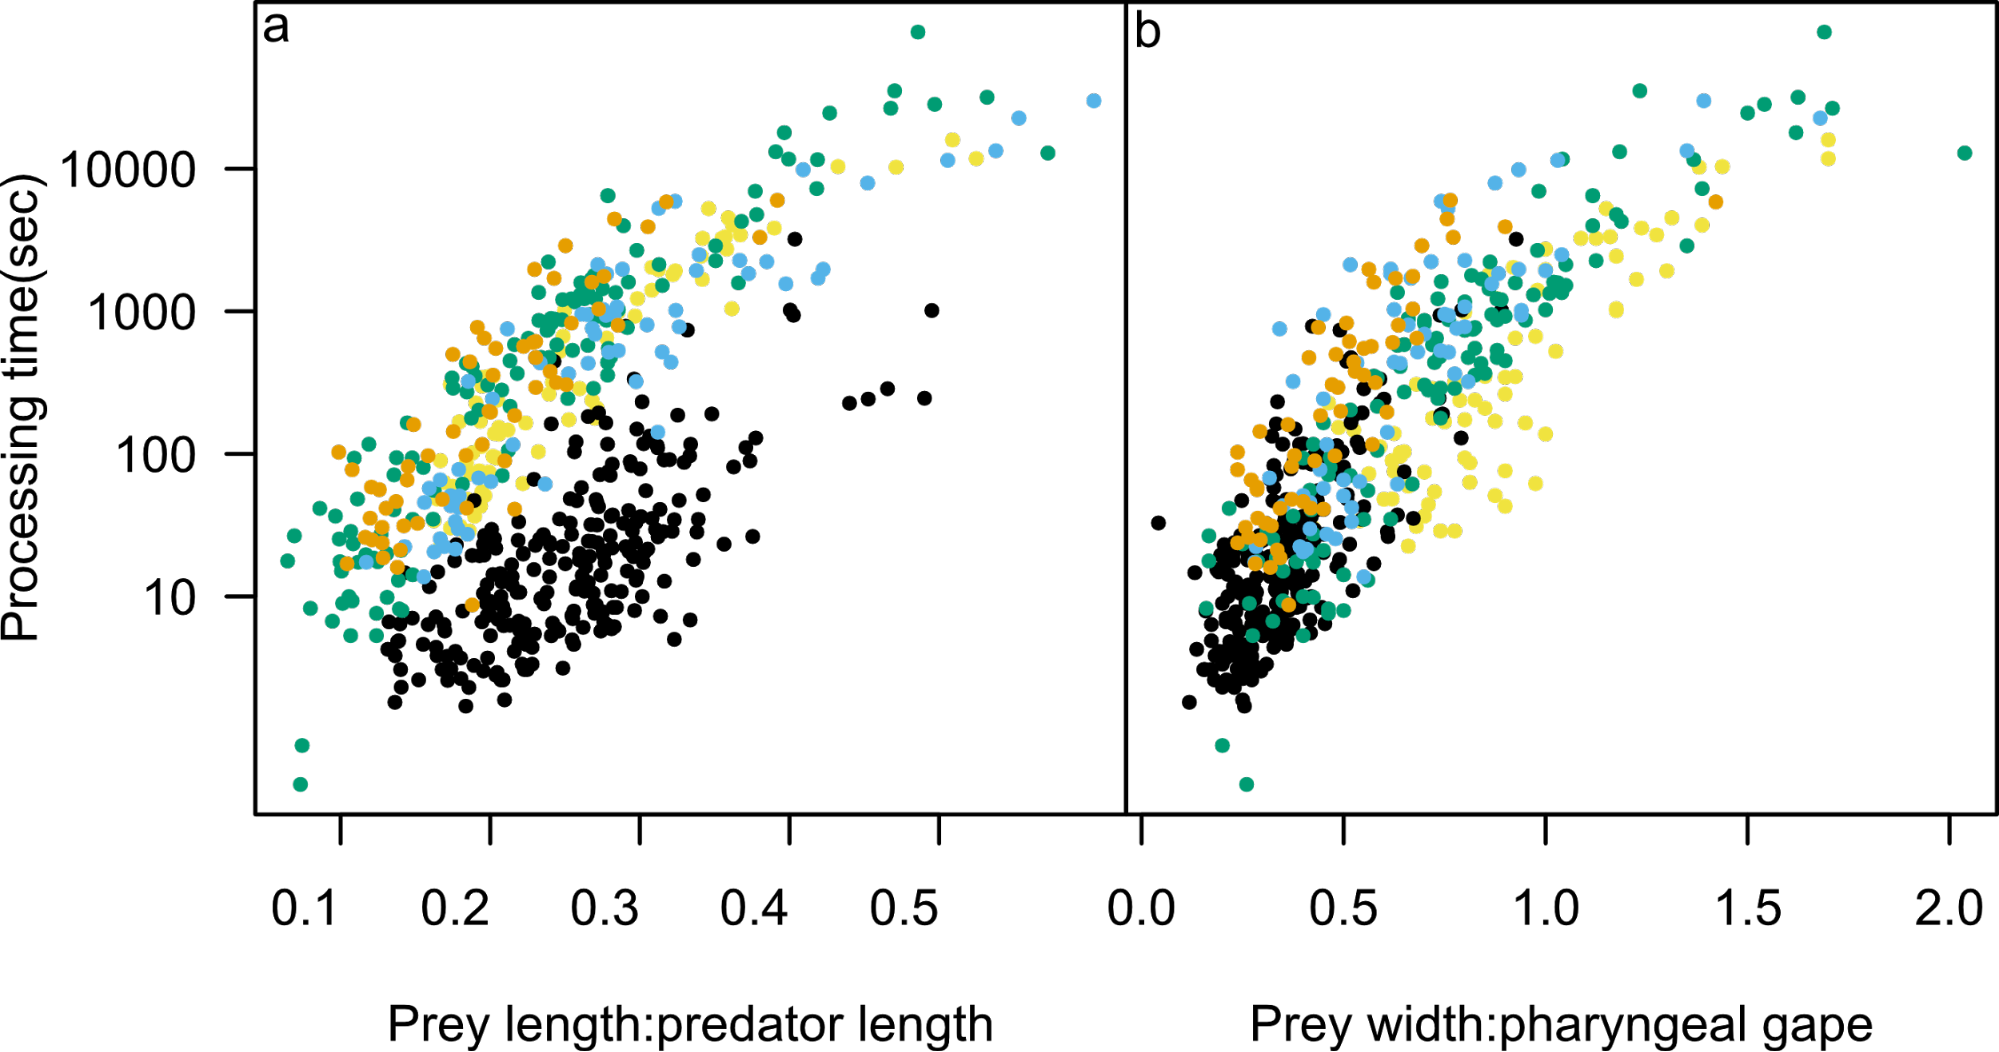
\includegraphics[width=\textwidth]{FishJaws/figures/fig5}
    \caption{\textbf{Prey processing times relative to body size and pharyngeal gape.} Pharyngeal processing time \textbf{(a)} with respect to predator length, as in Figure \ref{FJ_fig2}b, or \textbf{(b)} with respect to pharyngeal gape. Black circles represent Nile perch trials, colored circles represent Victorian haplochromine trials corresponding to species in Figure \ref{FJ_fig1}a.}
    \label{FJ_fig5}
\end{figure}

\subsection{Historical extinction patterns}

We recorded extinction and ecological data \cite{redlist} for 73 species of Victorian cichlid fish from the Mwanza Gulf (Table \ref{FJ_table3}). We scored cichlid species seen in survey trawls after the 1980s as not extinct, and fish not seen since the 1980s or earlier as extinct. We also recorded whether fish occurred at littoral depth (0-6m), sublittoral (6-20m), and/or offshore depth (greater than 20m). We recorded whether fish occurred over mud, sand, rocks, and whether or not the fish occurred in open water. We also recorded whether fish ate rock algae, phytoplankton, detritus, zooplankton, insects, snails, fish, cichlid eggs/larvae, fish scales, decapods, or external parasites. For body size measurements for species described after 1950, we recorded maximum standard length from the species descriptions. \cite{greenwood1981haplochromine, witte1980haplochromine, hoogerhoud1982ecological, van1991systematic, van1992haplochromis, van1996taxonomical, seehausen1996lake, seehausen1998mbipi, van2004haplochromis, seegers2008fishes, van2008haplochromis, de2010seven, de2013two} For species described earlier than the 1950s, we used published measurements of maximum size from the Checklist of Freshwater Fishes of Africa (CLOFFA). \cite[p. 100-184]{daget1991check} Species with standard length greater than the average were scored as having a large body size, and fish equal or below average were scored as small body size.
	
We then examined which of our ecological variables was most important for describing extinction patterns in the lake using a machine learning approach, conditional inference forests, \cite{hothorn2006unbiased} a variant of the popular random forest technique for machine learning. In order to assess variable importance, we utilize an AUC-based (not to be confused with AIC) metric that assesses how the area underneath the receiver operating curve (AUC), a metric of prediction importance, changes when the variable in question is randomly permuted. Important variables degrade noticeably when randomly permuted, causing a high mean decrease in accuracy, while unimportant predictors will not change or even increase when randomly permuted, causing low or negative mean decrease in accuracy. Conditional inference forests with AUC-based importance metrics can currently handle both class imbalance and correlated predictors better than both typical random forest methods and other importance metrics like the Gini coefficient. \cite{hothorn2010party} All conditional inference forest analyses were performed using the R package 'party,' \cite{janitza2013auc} using default parameters, 10,000 trees, and 100 permutations.

We find that a fish diet is the most important predictor of extinction, followed by presence in the rocky habitat and body size, respectively. Occupancy of the rock habitat and small body sizes have been shown to reduce the likelihood of extinction in previous studies, \cite{witte_destruction_1992, seehausen1997patterns} but this is the first time a fish diet has been shown to correlate with increased extinction risk in Lake Victoria. Relaxed mating selection and increased rates of interspecific hybridisation, mediated by eutrophication-driven turbidity, has been shown to be partially responsible for the collapse of cichlid species diversity, \cite{seehausen1997patterns} and it is possible that presence at rocky islands, one of our predictor variables, represents not just refuge from the Nile perch \cite{witte_destruction_1992} but also refuge from effects of eutrophication. \cite{witte_destruction_1992, witte2013cichlid} However, species loss by hybridization cannot explain the near-complete elimination of piscivorous cichlids including offshore islands with clear water. Eutrophication has been suggested to affect competition between visually hunting predators because it is expected to lead to dietary convergence[68, and this may have strengthened competition between predatory cichlids and Nile perch, but -- by itself -- it does not predict the rapid displacement of nearly all predatory cichlids by Nile perch, nor the pronounced morphological shift in the community of relict piscivores caught in recent years (see below).

\subsection{Morphological variables predicting piscivory}

For all but two of the Lake Victoria cichlid species which had no published morphological data available ({\em Paralabidochromis crassilabris}, {\em H. perrieri}), we also recorded standard length, lower jaw length, head length, and body depth from the species descriptions. \cite{greenwood1981haplochromine, wagner2013genome, schwartz2006effects, hoyle1987effect, bates2010lme4, kuznetsova2013lmertest, redlist, witte1980haplochromine, hoogerhoud1982ecological, van1991systematic, van1992haplochromis, van1996taxonomical, seehausen1996lake} If mean values were available, we used those, otherwise measurements from the holotype were used, or the midpoint of the smallest and largest values of trait. If measurements were expressed as a ratio with head length or standard length, we converted them back to raw distances. We then corrected for interspecific size variation with a $\log_{10}$-$\log_{10}$ regression on standard length. If not, we used the midpoint between the largest and the smallest fish. We used a machine learning framework identical to that described above to examine which of our four phenotypic variables was the most important predictor of a fish diet, and found that size-corrected lower jaw length was the most important predictor (Figure \ref{FJ_fig6}), followed by head length. 

\begin{figure}
    \centering
    
\includegraphics[width=4in]{FishJaws/figures/fig6}
    \caption{Lower jaw length best predicts piscivory in Victorian cichlids. Importance analysis for size-corrected morphological variables predicting piscivory in 68 of the 72 species used in the ecological analysis.}
    \label{FJ_fig6}
\end{figure}

\subsection{Morphological shifts in fish-eating cichlid communities}

We measured lower jaw length and standard length for all described species of Lake Victoria fish-eating cichlid (Table \ref{FJ_table4}) as indicated by Witte and van Oijen \cite{witte1990taxonomy} and any subsequent descriptions of fish-eating species. \cite{van1991systematic, van1992haplochromis, van2004haplochromis, van2008haplochromis} We also measured the same variables in Victoria Basin Nile perch juveniles ($n=80$) from the Florida Museum of Natural History collection comprising the same size range as Victorian cichlid piscivores from the Victoria Basin. These fish are taken to be representative of both Victoria Basin and Tanganyikan {\em Lates} species, as a review \cite{greenwood1976review} of the genus {\em Lates} indicated that lower jaw length is not variable between species of {\em Lates}. We also measured a set of relict Victorian piscivores ($n=27$) and one representative of each known evolutionary transition to piscivory in Tanganyikan cichlids. All measurements were from formalin-fixed specimens later transferred to ethanol.

\begin{figure}
    \centering
    \begin{subfigure}[t]{2.8in}
        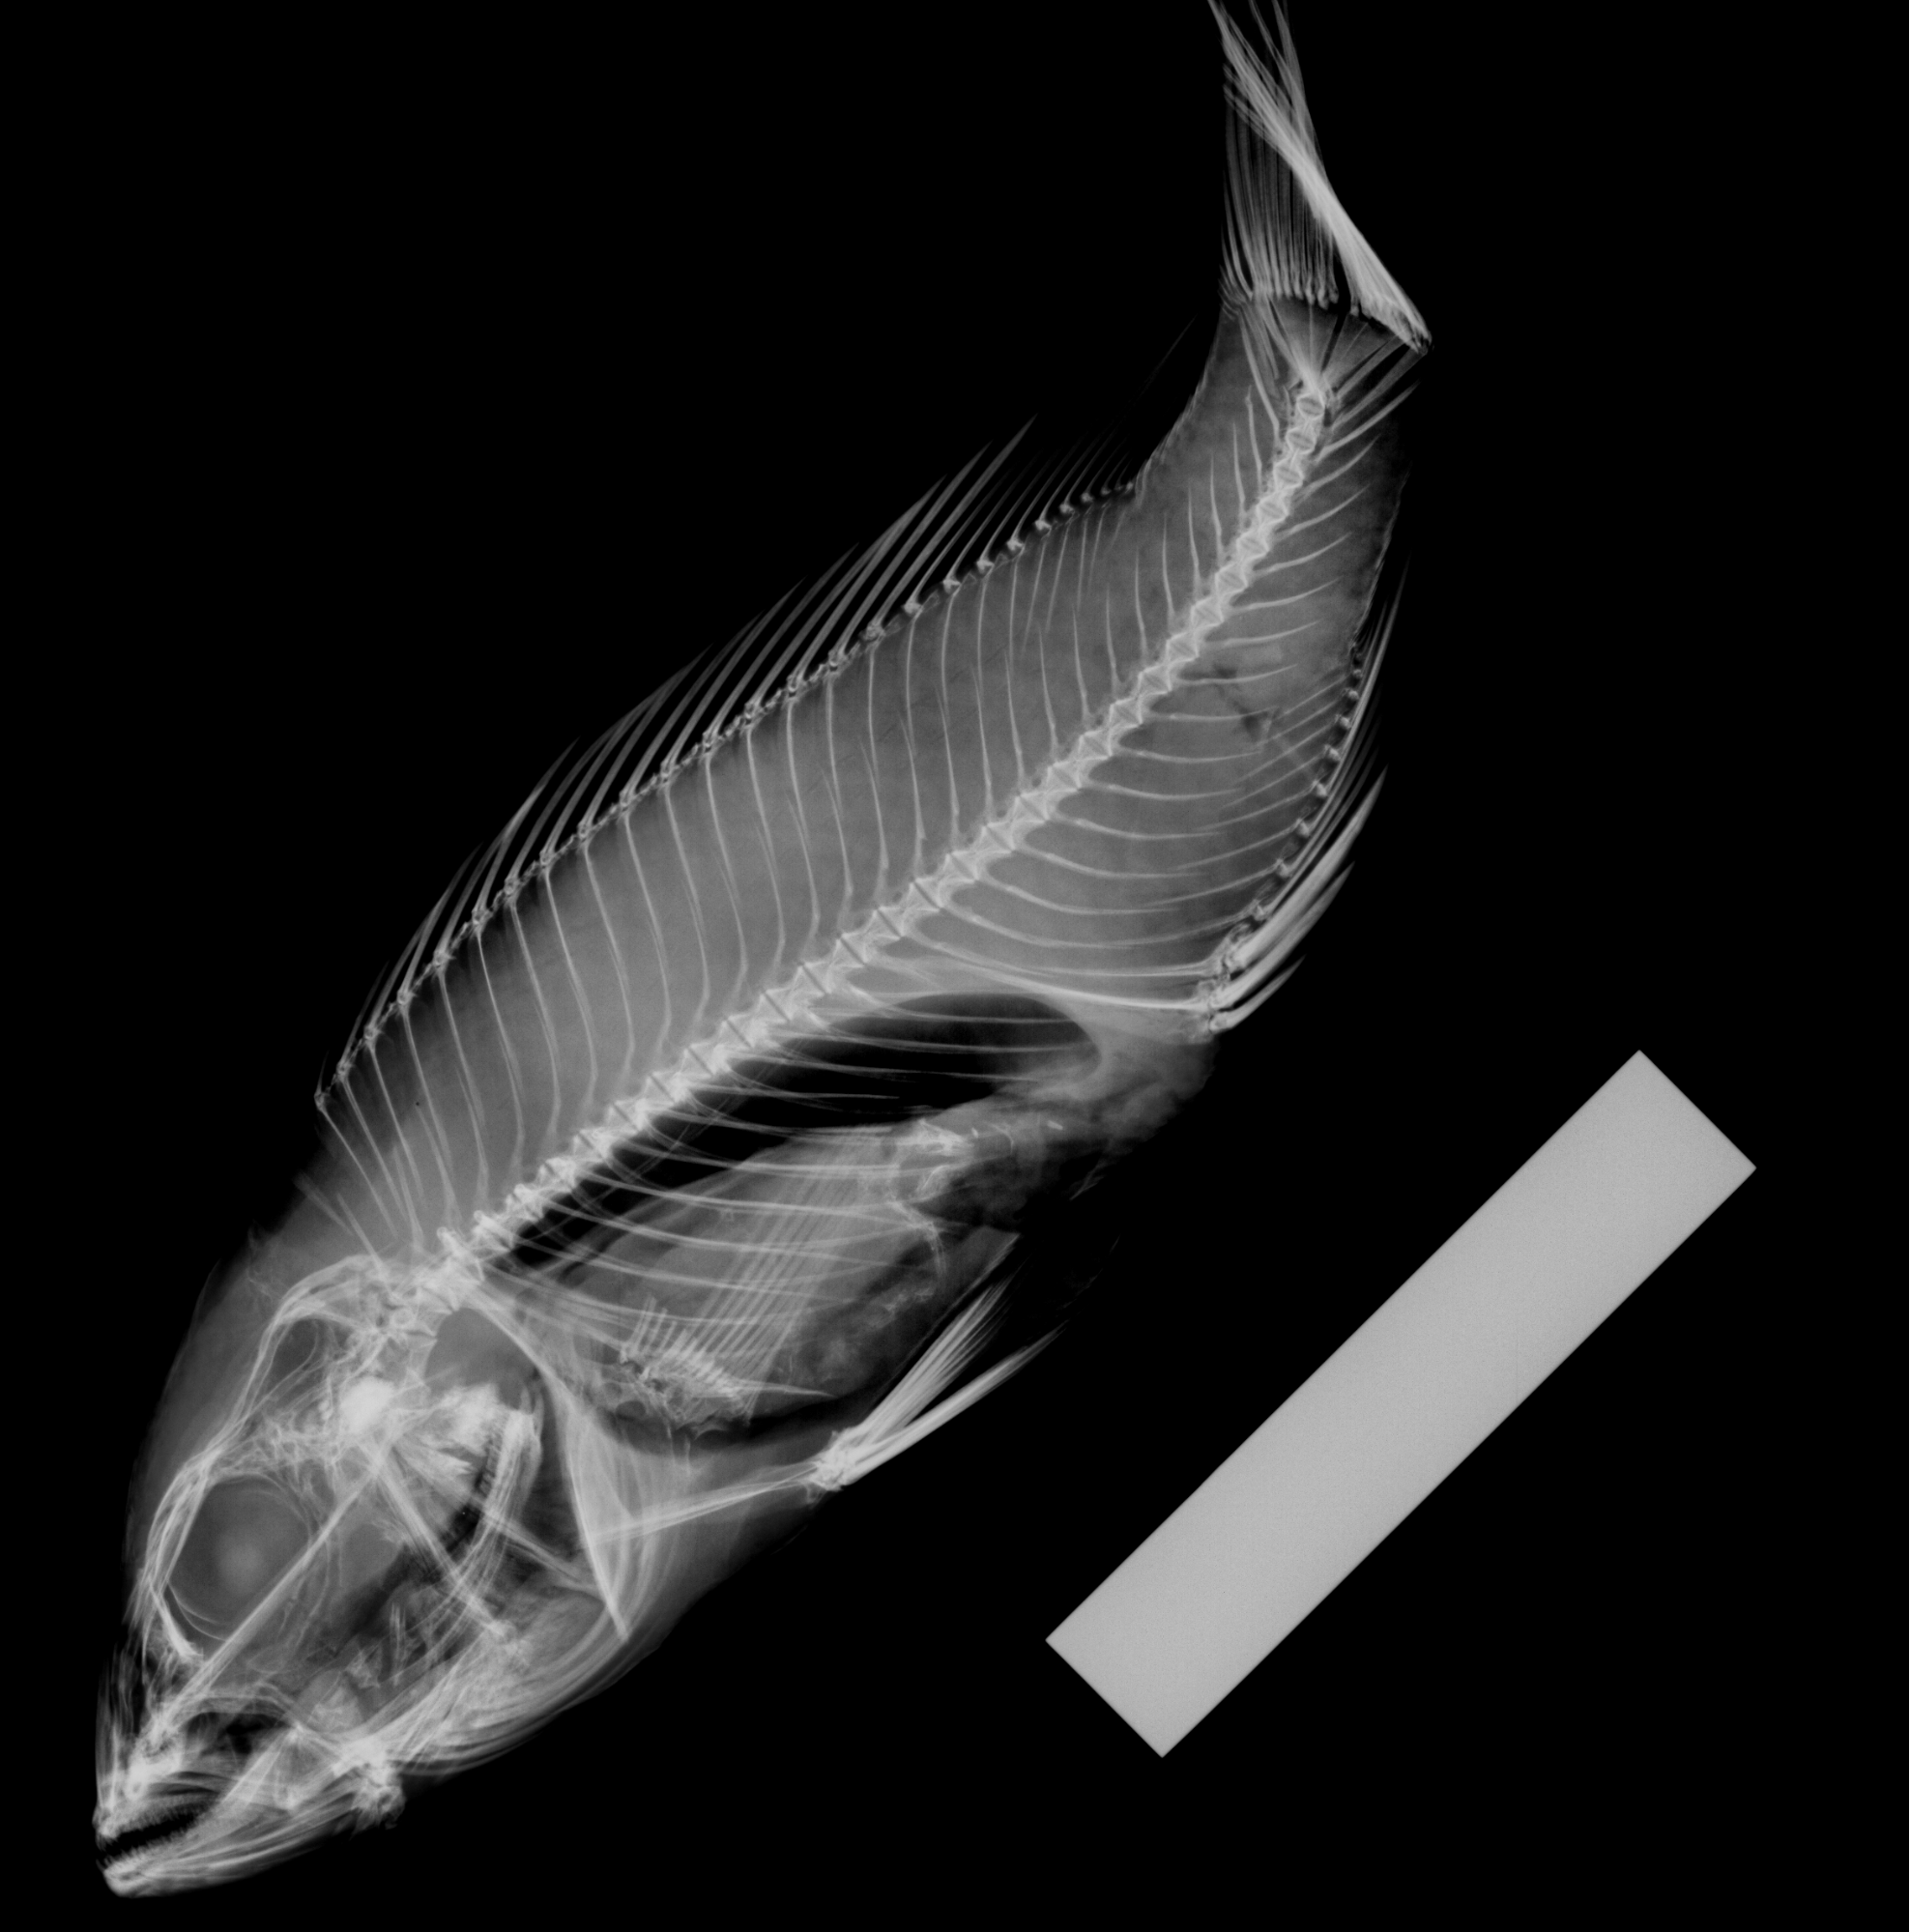
\includegraphics[width=2.8in]{FishJaws/figures/fig7a}
    \end{subfigure}
    \begin{subfigure}[t]{2.8in}
        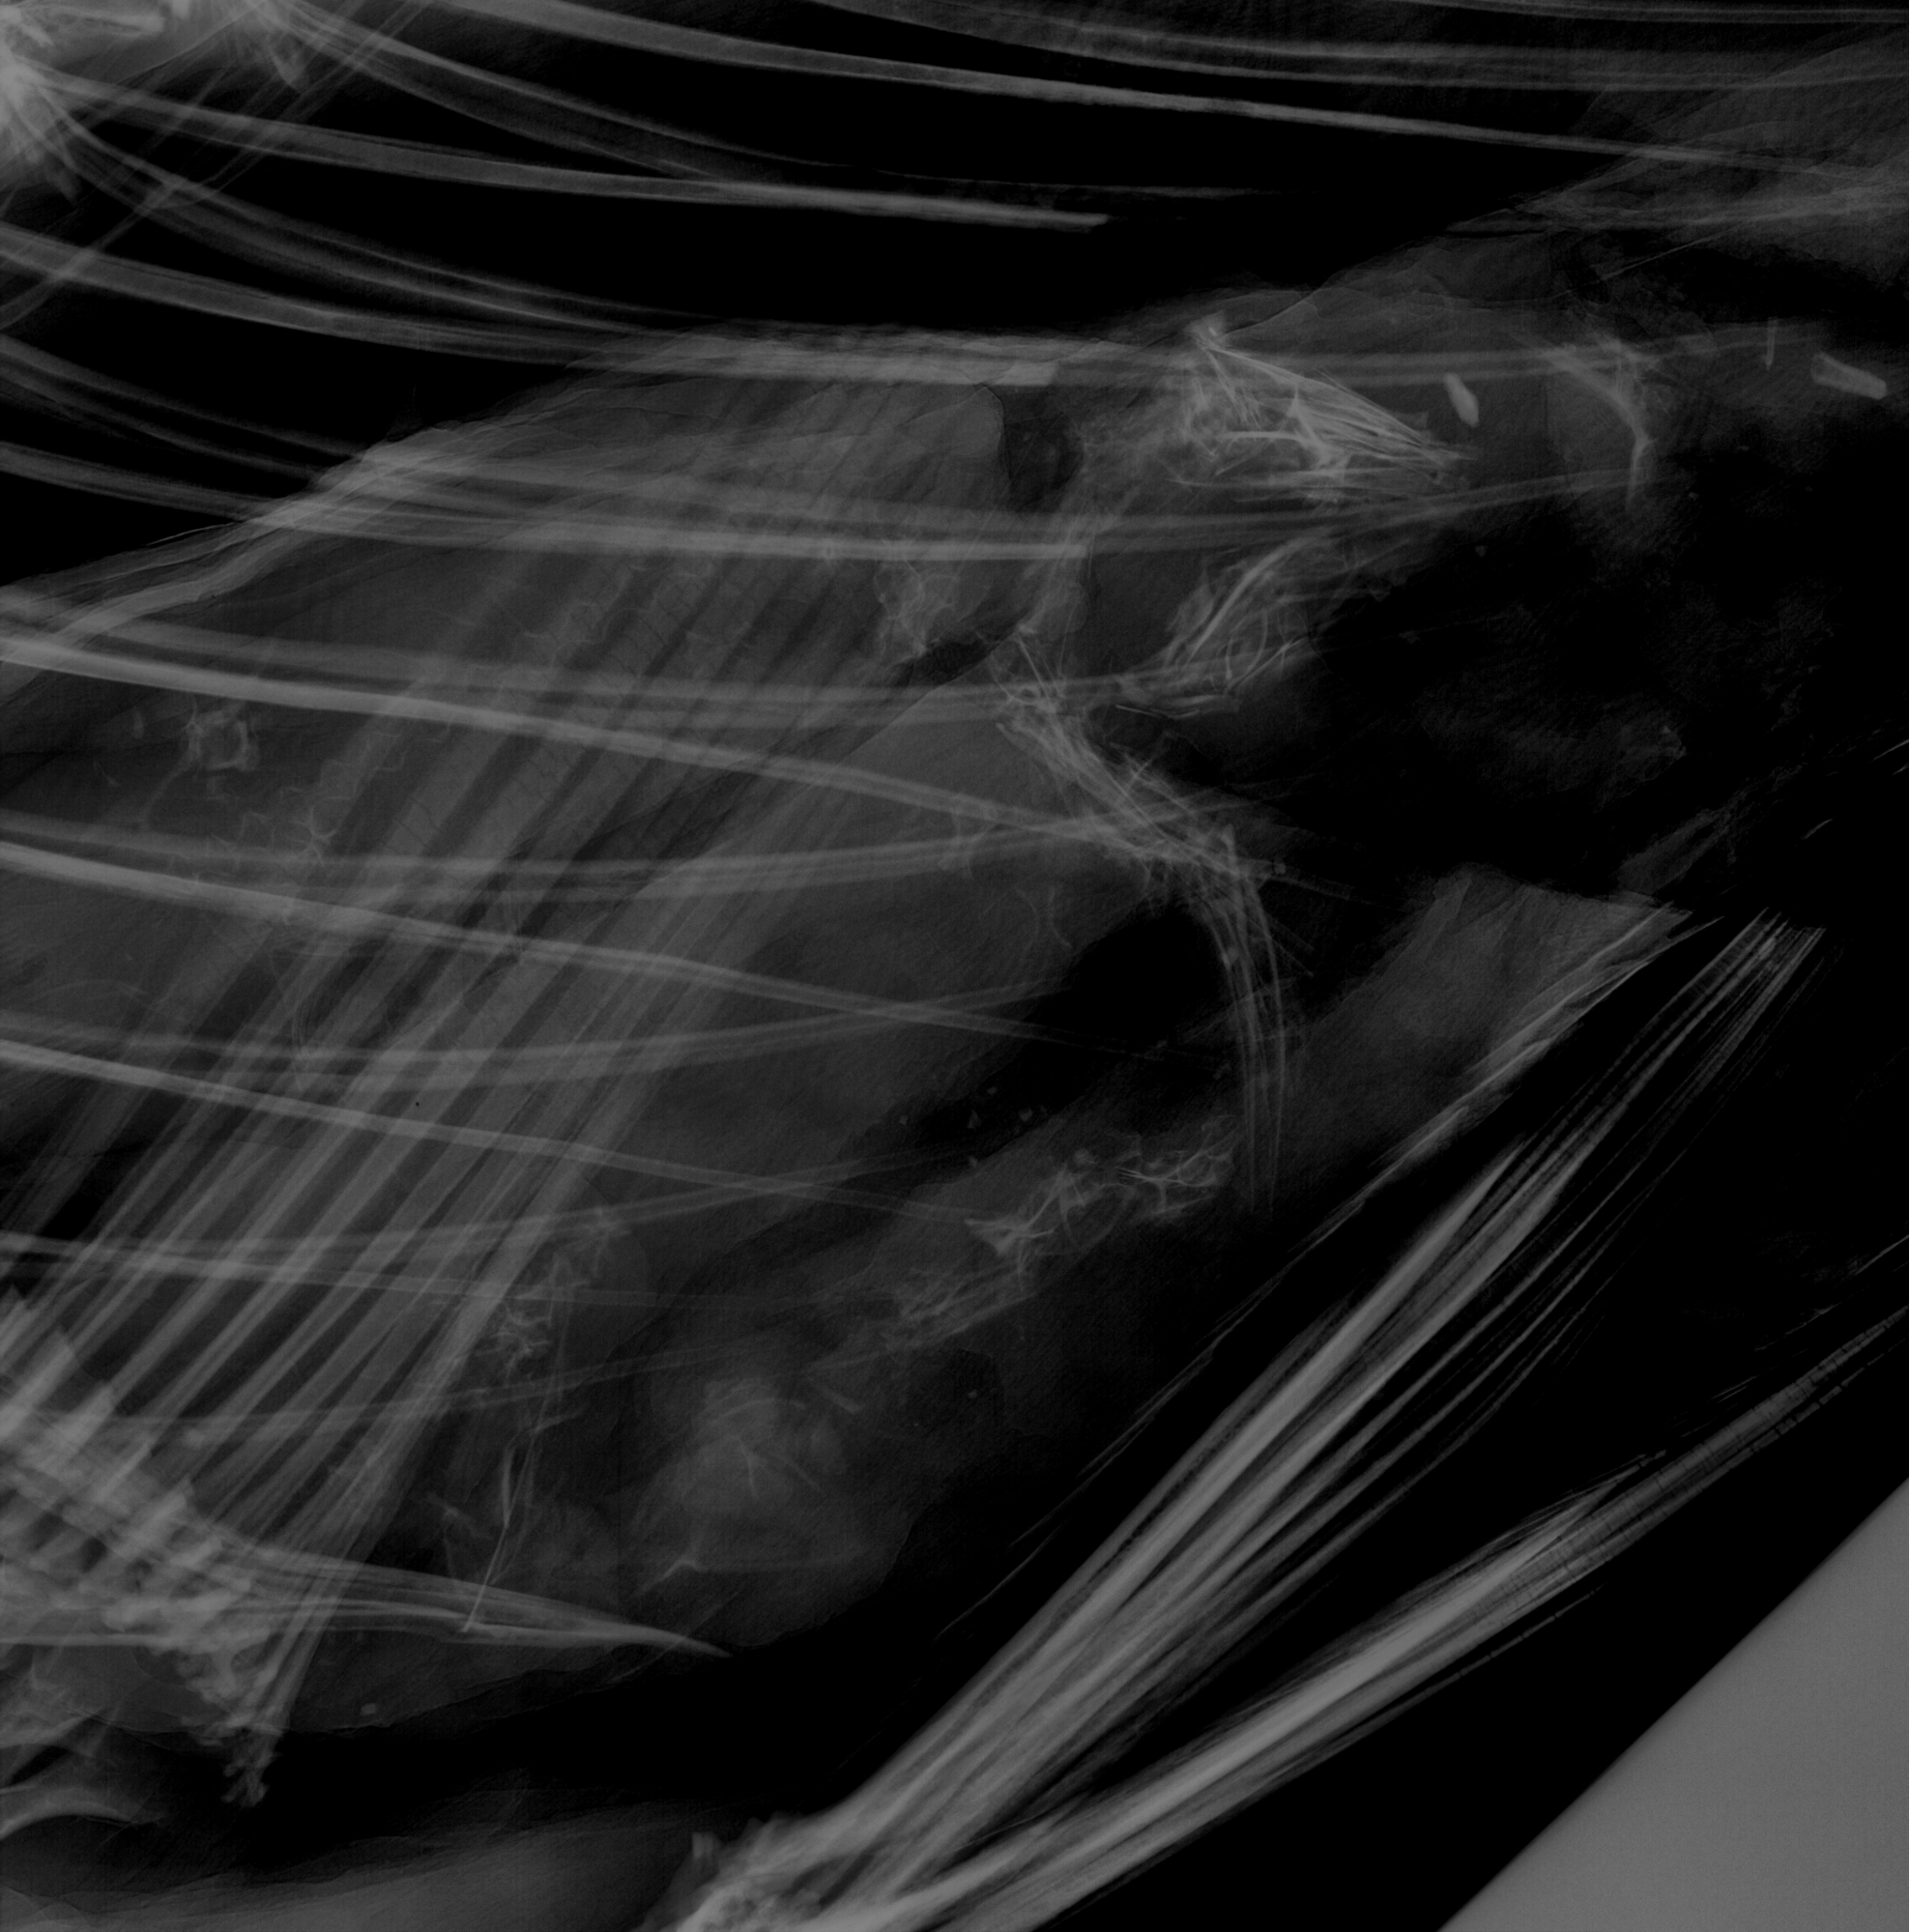
\includegraphics[width=2.8in]{FishJaws/figures/fig7b}
    \end{subfigure}
    \caption{\textbf{Stomach contents of a relict piscivore from Lake Victoria.} X-ray of example relict piscivore ({\em Harpagochromis} sp.) and stomach contents showing fish remains, with 5cm bar for scale.}
    \label{FJ_fig7}
\end{figure}

Relict piscivores were collected over several field expeditions to the Mwanza and Speke Gulf of Lake Victoria (Tanzania) from the period 2005 to 2010. From those expeditions, 73 individuals were visually identified as belonging to the piscivorous genera {\em Harpagochromis} and {\em Prognathochromis}. To verify that these fish were still piscivorous and had not transitioned to an alternative diet, as in some other groups of Victorian cichlids post-invasion, \cite{kishe2008dietary} we then X-rayed the gut contents of each fish. Out of the 73 individuals we identified 27 with fish bones in the gut and these were retained for the morphological analysis described above. These individuals were difficult to sort into `species' in many cases, but results do not differ if they are treated only as individuals or grouped into loose species designations first.

We size corrected lower jaw length across all individuals with residuals taken from a $\log_{10}$-$\log_{10}$ regression on standard length. Many of the Tanganyikan piscivores are closely related, so we split the species into eight independent transitions (Table \ref{FJ_table5}). If piscivory only evolved once within a tribe, it was assumed to be independent from other evolutionary transitions to piscivory within Tanganyika. One tribe, Lamprologini, contains several piscivorous genera, so we used the latest lamprologine phylogeny \cite{sturmbauer2010evolutionary} to determine which of these were likely to be independent transitions. We identified three: the large rock-dwelling predators in the genus {\em Lepidiolamprologus}, the ambush predator {\em Lamprologus lemairii}, and the sand-dwelling predator {\em Neolamprologus cunningtoni}. If a piscivore transition contained only one species, we used the species mean of size-corrected lower jaw length for that species. If a group contained a species pair, we averaged the species means of size-corrected lower jaw length for that pair. If a group contained three or more species (Table \ref{FJ_table6}), we obtained ND2 sequences of those species from Genbank, then produced a small ultrametric tree of the species using maximum-likelihood and the {\tt Timetree} function in the program {\tt MEGA6} using default parameters. \cite{tamura2013mega6} We then calculated the phylogenetic mean of size-corrected lower jaw length for each independent evolution of piscivory in Tanganyika using the {\tt fastAnc} function in the {\tt phytools} \cite{revell2012phytools} {\tt R} package.

We then used a pairwise Wilcox test in R to compare Nile perch, pre-invasion Victorian piscivores, post-invasion Victorian piscivores, and Tanganyikan piscivore groups to each other, using a Holm correction to account for multiple comparisons. Nile perch have larger jaw sizes than all three cichlid populations ($p<0.001$ for all). The pre-invasion Victorian fish-eaters have a larger jaw than the post-invasion relict Victorian fish-eaters ($p<0.0001$). The Tanganyikan fish-eaters have a smaller mean than the pre-invasion fish-eaters of Lake Victoria ($p<0.025$) but do not differ from the post-invasion fish-eaters of Lake Victoria ($p=0.65$). While most Tanganyika cichlid predators have relatively small jaws, it is notable that one transition to piscivory has a very similar lower jaw length to the Nile perch species mean. This transition involves a single species, {\em Lamprologus lemairii}, which possesses a very different predatory ecology relative to Nile perch. Specifically, it is a demersal sit-and-wait predator similar to a coral reef scorpionfish, not an active hunter like Nile perch (Figure S5). 

\begin{figure}
    \centering
    \begin{subfigure}[t]{2.8in}
        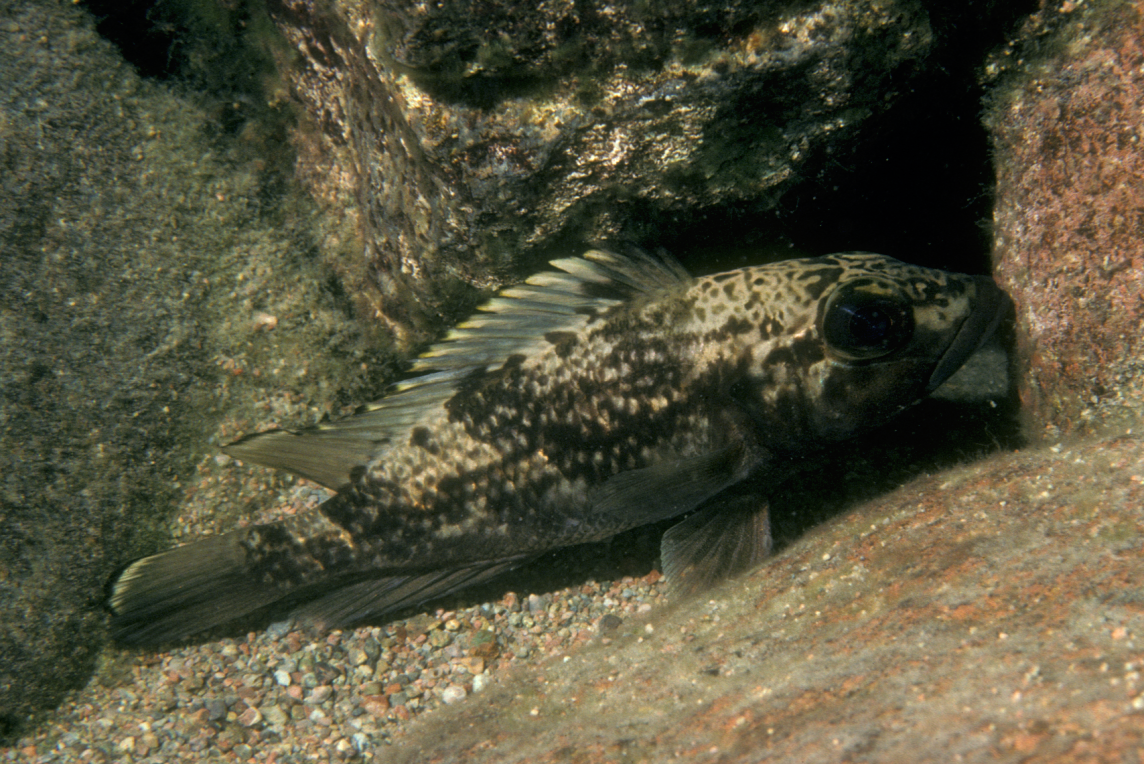
\includegraphics[width=2.8in]{FishJaws/figures/fig8a}
    \end{subfigure}
    \begin{subfigure}[t]{2.8in}
        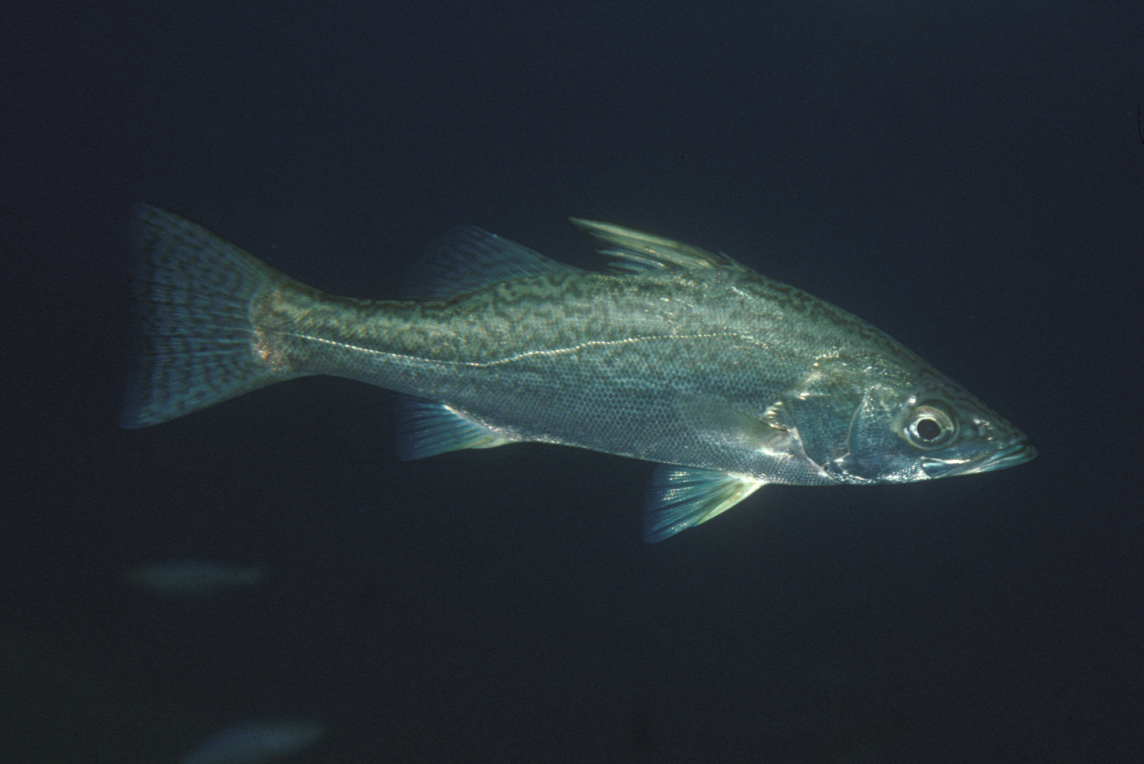
\includegraphics[width=2.8in]{FishJaws/figures/fig8b}
    \end{subfigure}
    \caption{\textbf{Divergent predation strategies of {\em Lamprologus lemairii} and predatory {\em Lates}.} Underwater photographs of \textbf{(a)} {\em L. lemairii} and \textbf{(b)} Tanganyikan {\em Lates}, two lineages with very different predatory strategies. {\em L. lemairii} is a sedentary sit-and-wait predator, while {\em Lates} is an active hunter. Photos taken by H. Buescher.}
    \label{FJ_fig8}
\end{figure}


\subfile{FishJaws/table1}
\subfile{FishJaws/table2}
\subfile{FishJaws/table3}
\subfile{FishJaws/table4}
\subfile{FishJaws/table5}
\subfile{FishJaws/table6}
